\documentclass[submit,techreq,noauthor]{eco}	% semi style
\usepackage[dvips]{graphicx}
\usepackage{listings, jlisting} 		% for source code
\usepackage{url}
\usepackage{setspace}
\usepackage{here}
%\setstretch{1.5} % 行間を広くします(資料チェックしてもらうときはコメントを外す)

\lstset{
  basicstyle={\ttfamily},
  identifierstyle={\small},
  commentstyle={\smallitshape},
  keywordstyle={\small\bfseries},
  ndkeywordstyle={\small},
  stringstyle={\small\ttfamily},
  frame={tb},
  breaklines=true,
  columns=[l]{fullflexible},
  numbers=left,
  xrightmargin=0zw,
  xleftmargin=3zw,
  numberstyle={\scriptsize},
  stepnumber=1,
  numbersep=1zw,
  lineskip=-0.5ex
}

\begin{document}

\semino {5/25}					% 年度/回数
\date   {5/07/18/火}				% 平成/月/日/曜日
\title  {ライブラリ関数単位でのプログラムへの影響と\\システムコールの比較2}	% タイトル
\author {奥 若菜}				% 氏名


\begin{abstract}
	Linuxマシンが製品やサービスの基盤として広く利用されるようになっていることで,それを標的とするLinuxマルウェアが劇的に増加している.
  また,Linuxマルウェアの開発動向として,マルウェアが自身の攻撃をセキュリティソフトに検知されないようにする回避技術の大幅な向上が確認されている.
  2021年に発見されたマルウェアSymbioteは,一般的に見られるLinuxマルウェアと比較して,極めて検出が困難とされる.
  SymbioteはLD\_PRELOADを使用して,すべての実行中のプロセスにロードされる共有ライブラリとして動作し,
  正当なプロセスの下で自身や他のマルウェアの痕跡を隠蔽する.
  本研究では,Symbioteのような共有ライブラリを用いた攻撃を行うマルウェアを動的解析し,その挙動を明らかにするとともに,効果的な検知手法の発見を目指す.
  前回までは,Symbioteを静的解析することで,エクスポートされるライブラリ関数の役割や隠蔽されるファイル名・プロセス名を特定した.
  今回は,Symbioteのライブラリ関数を使用するプログラムを実行したときの実行結果とシステムコールの差分を,実行時の条件ごとに収集した.
  その結果,Symbiote感染時であっても,ライブラリ関数ごとに特定の条件を満たしたときのみ,出力結果やシステムコールに変化が現れる場合があることがわかった.
\end{abstract}
\maketitle


\section{はじめに}
IoTデバイスの普及や企業のクラウドシフトにより,製品やサービスの基盤として,Linuxマシンを利用するケースが増えた.
攻撃対象が広がったことで,それを標的とするLinuxマルウェアも劇的に増加している\cite{TREND-MICRO}.
Linuxマルウェアの開発動向としては,マルウェアが自身の攻撃をセキュリティソフトに検知されないようにする回避技術の大幅な向上が確認されている\cite{IBM}.
%Linuxマルウェアの技術革新の水準はWindowsベースのマルウェアに迫る勢いとされ,この傾向は2022も高まると予想されている.
このことから,今後もより高度な潜伏機能を持つマルウェアが開発される可能性が高く,対策を怠ると重大な被害に繋がると考えられる.


2021年に発見されたSymbioteは,Linuxで一般的に見られるマルウェアとは異なる特徴を持ち,極めて検出が困難とされる\cite{Symbiote}.
Symbioteは,単独の実行可能ファイルではなく,LD\_PRELOADによってすべての実行中のプロセスにロードされる共有ライブラリとして動作する.
LD\_PRELOADとは,Linuxにおいて,プログラム実行時に共有ライブラリを動的リンクするために使用される環境変数である.
Symbioteは,LD\_PRELOADを使用することで,プログラムによって要求される正当な共有ライブラリの代わりに,悪意のある共有ライブラリを提供する.
このように悪意のある共有ライブラリをプログラムにロードし,不正なコードを実行する攻撃をDynamic Linker Hijackingという\cite{MITRE-ATT&CK}.
この攻撃では正当なプロセスの下で,注入されたコードの実行が隠されるため,プロセスベースの解析は回避される可能性が高い.

本研究は,動的解析を行うことによってSymbioteの挙動を明らかにすることを目指す.
また,SymbioteのようなDynamic Linker Hijackingを行うLinuxマルウェアの効果的な検知手法および対策方法を考察する.


以下,2章でSymbioteの機能を説明し,3章で解析を行う検体とそのライブラリ関数について説明する.
4章でシステムコールトレースによる動的解析の結果を述べ,5章でまとめる.\\


\section{Symbioteの機能}
Symbioteが初めて検知されたのは2021年11月であり,
ラテンアメリカの金融セクターを標的とするために作成されたとされている.
Symbioteについての調査は,Intezerの研究者Joakim KennedyとBlackBerryのResearch and Intelligence Teamによって
行われ,レポートが作成されている.以下に文献\cite{Symbiote}のレポートをもとにSymbioteの機能を示す.


\subsection{検知回避機能}
Symbioteは,LD\_PRELOADで指定した共有ライブラリによって,プログラムによる関数の呼び出しをフックし,
悪意のあるコードを実行することで,検知を回避する.具体的には,C言語の標準ライブラリであるlibcおよび
パケットキャプチャのためのライブラリであるlibpcapの関数をフックすることで,以下のような回避機能を実現する.
  \begin{description}
    \item [プロセスの隠蔽] \mbox{}\\
    呼出し元のアプリが/proc以下にあるファイルまたはディレクトリにアクセス
    しようとすると,プロセス名を元に出力を消去する.
    \item [ファイルの隠蔽] \mbox{}\\
    呼出し元のアプリが上記以外の場所にアクセスしようとすると,暗号化さ
    れたファイルリストにある名前を元に出力を消去する.
    \item [ネットワークトラヒックの隠蔽] \mbox{}
      \begin{description}
        \item[UDP:] 
        libpcapライブラリの関数をフックし,受信したパケットごとにドメインの文字列をチェックする.一致した場合はそのパケットをスキップして呼出し元に返す.
        \item[TCP:] 
        fopenとfopen64をフックし,プロセスがproc/net/tcpを開こうとすると,該当するポートをスキップして呼出し元に返す.
        感染マシンがeBPFを使用してパケットキャプチャを行う場合は,setsockoptをフックし,提供されたeBPFコードの前に独自のバイトコードを付加することで,ポートに基づきパケットを消去する.
      \end{description}
  \end{description}

\subsection{ルートキット機能}
Symbioteはすべての実行中のプロセスに感染した後,認証情報を収集し,攻撃者にリモートアクセスなどのルートキット機能を提供する.

認証情報の収集は,sshやscpプロセスによって呼び出されるlibcのread関数をフックすることで行われる.
収集した認証情報はファイルに書き込まれるだけでなく,
16進エンコードされ,攻撃者が運用するサーバにDNSのAレコード要求を通じて持ち出される.\\
\indent
感染したマシンへのリモートアクセスは,Pluggable Authentication
Module(PAM)機能を提供するlibpamの関数をフックすることで提供される.アプリケーション(telnetやssh)がPAMを利用してユーザを認証する際に,攻撃者のあら
かじめ設定したものと同じ認証情報でアクセスすると,フックされた関数が成功応答を返すとともに,攻撃者もアクセスが可能になる.

\subsection{緊急アクセス機能}
Symbioteは通常のプロセスが機能しない場合に,攻撃者のC\&CサーバにDNSのTXTレコード要求を送信し,マシンへの緊急アクセスを
提供する.TXTレコードの形式は,\%MACHINEID\%.\%C\&C\_DOMAIN\%となっている.応答を取得すると,このマルウェアはコンテンツをbase64
デコードし,コンテンツが正しいed25519秘密鍵で署名されているかどうかをチェックし,
RC4でコンテンツを復号して,生成されたbashプロセスでシェルスクリプトを実行する.\\


\section{解析を行う検体とライブラリ関数}
\subsection{検体}
マルウェア分析プラットフォームであるIntezer AnalyzeとVirusTotalを用いてSymbioteを探索したところ,表\ref{table: Artifact}に示す6検体が見つかった.
これらはIntezerのレポートに記載されている検体のハッシュと一致しており,更新情報もないため,現在まででSymbioteとされている検体は,この6検体が全てである可能性が高い.\\
アップロード日の項目には,Intezer Analyzeへ検体がアップロードされた日付を示す.ファイル名の項目には,攻撃者によって検体ファイルに設定されると想定される名前を示す.
また,ライブラリ関数の項目には検体の共有ライブラリによってエクスポートされる関数の数を示す.\\
\indent
6検体のうち,検体4のみが実行ファイルであり,実行を開始すると2.3節で述べた緊急アクセス機能を提供する.
その他の検体は,すべて共有ライブラリファイルであり,LD\_PRELOADに検体ファイルのパスを設定することで動作する.
動的解析による共有ライブラリの影響調査は,主に最新の検体である検体6を使用する.検体6で実装されていないライブラリ関数については,次に新しい検体5を使用する.

\subsection{検体がエクスポートするライブラリ関数}
Symbioteの共有ライブラリはELFファイルであるため,readelfコマンドを用いてライブラリ関数のシンボル情報を
取得できる.表2は,Symbioteの5つの共有ライブラリについて,エクスポートされるライブラリ関数の一覧を示す.丸がついているライブラリ関数は,その検体からエクスポートされることを表している.
影響調査は,最新の検体である検体6で実装されているライブラリ関数を全てと,3つ以上の検体で実装されているライブラリ関数を合計した16種類の関数について行う.\\


\begin{table*}[t]
  \caption{Symbioteの検体とファイル名一覧}
  \label{table: Artifact}
  \centering
  \begin{tabular}{|c|c|c|c|}
  \hline
  No. & hash256                                                                                                        & アップロード日 & ファイル名 \\ \hline
  1   & \begin{tabular}[c]{@{}l@{}}121157e0fcb728eb8a23b55457e89d45\\ d76aa3b7d01d3d49105890a00662c924\end{tabular} & 2021/11/27 & kerneldev.so \\ \hline
  2   & \begin{tabular}[c]{@{}l@{}}f55af21f69a183fb8550ac60f392b05d\\ f14aa01d7ffe9f28bc48a118dc110b4c\end{tabular} & 2022/01/19 & mt64.so \\\hline
  3   & \begin{tabular}[c]{@{}l@{}}ec67bbdf55d3679fca72d3c814186ff4\\ 646dd779a862999c82c6faa8e6615180\end{tabular} & 2022/01/26 & search.so \\ \hline
  4   & \begin{tabular}[c]{@{}l@{}}45eacba032367db7f3b031e5d9df10b\\ 30d01664f24da6847322f6af1fd8e7f01\end{tabular} & 2022/01/29 & dnscat\\ \hline
  5   & \begin{tabular}[c]{@{}l@{}}a0cd554c35dee3fed3d1607dc18debd\\ 1296faaee29b5bd77ff83ab6956a6f9d6\end{tabular} & 2022/02/01 & liblinux.so \\ \hline
  6   & \begin{tabular}[c]{@{}l@{}}cb4bbe3af754779e673c6ae84cb38d7f\\ 2ccbc9a1d59c52abbb98451d070dba3c\end{tabular} & 2022/08/19 & libpcap3.so \\ \hline
  \end{tabular}
\end{table*}


\begin{table*}[t]
  \caption{エクスポートされるライブラリ関数一覧}
  \label{table: library}
  \centering
  \begin{tabular}{|c|c|c|c|c|c|}
  \hline
  ライブラリ関数           & kerneldev.so & mt64.so & search.so & liblinux.so & libpcap3.so \\ \hline
  \_fini            & ○            & ○       & ○         & ○           & ○           \\ \hline
  \_init            & ○            & ○       & ○         & ○           & ○           \\ \hline
  fopen,fopen64     & ○            & ○       & ○         & ○           & ○           \\ \hline
  readdir,readdir64 & ○            & ○       & ○         & ○           & ○           \\ \hline
  fstatat,fstatat64 &              & ○       & ○         & ○           & ○           \\ \hline
  pam\_set\_item    & ○            & ○       & ○         & ○           & ○           \\ \hline
  pam\_acct\_mgmt   &              & ○       & ○         & ○           & ○           \\ \hline
  pam\_authenticate & ○            & ○       & ○         & ○           & ○           \\ \hline
  crc32b            & ○            &         &           &             &             \\ \hline
  RC4               & ○            &         &           &             &             \\ \hline
  recvmsg           &              & ○       & ○         & ○           & ○           \\ \hline
  pcap\_stats       &              & ○       & ○         & ○           & ○           \\ \hline
  pcap\_loop        &              & ○       & ○         & ○           & ○           \\ \hline
  setsockopt        &              & ○       & ○         & ○           & ○           \\ \hline
  download\_script  &              &         & ○         & ○           &             \\ \hline
  prepare\_pipe     &              &         & ○         & ○           &             \\ \hline
  read              & ○            & ○       & ○         & ○           & ○           \\ \hline
  execve            &              & ○       & ○         & ○           &             \\ \hline
  stat              &              & ○       & ○         & ○           & ○           \\ \hline
  statx             &              & ○       & ○         & ○           & ○           \\ \hline
  \end{tabular}
  \end{table*}



\section{ライブラリ関数ごとの特徴の収集}
検体を隔離環境で実行し,それぞれのライブラリ関数に対して,それを利用するプログ
ラムを実行したときの出力結果とシステムコールの差分を収集する.
4.1節で解析環境について説明し,4.2節で,Symbioteのライブラリ関数の分類と,独自の処理を行う条件を示す.4.3章で,それらの条件ごとに,出力結果とシステムコールの差分を示す.

\subsection{解析環境}
解析環境を構成するソフトウェアを表3に示す.
ゲストOSからホストおよびネットワークへのアクセスはできない.
また,検体の実行と解析は全てゲストOS上で行う.

\begin{table}[t]
  \caption{解析環境}
  \label{table: 解析環境}
  \centering
  \begin{tabular}{|l|l|}
  \hline
  Guest OS   & Ubuntu 22.04.2 LTS \\ \hline
  emulator   & QEMU 6.2.0         \\ \hline
  hypervisor & KVM                \\ \hline
  Host OS    & Ubuntu 22.04.2 LTS \\ \hline
  \end{tabular}
\end{table}

\subsection{Symbioteの処理が行われる条件}
ソースコードの静的解析により,Symbioteのライブラリ関数は,実行されたときの条件によって,処理の内容が変化するものとしないものがあると分かった.
また,実行時の条件によって処理の内容が変化するものには,条件によって,置き換えられた元のライブラリ関数をそのまま呼び出すだけの場合と,Symbioteの独自の処理を追加する場合があった.
Symbioteが独自の処理を行う場合を,条件を満たす場合とし,そうでない場合を条件を満たさない場合とする.動的解析を行う16種類のライブラリ関数について,条件を表4にまとめた.条件がなしとは,条件に関わらずSymbioteの独自の処理を行うライブラリ関数を表す.
\indent

\begin{table*}[t]
  \caption{ Symbioteの処理が行われる条件一覧}
  \label{table: 条件}
  \centering
  \begin{tabular}{|c|c|}
  \hline
  ライブラリ関数           & 条件\\ \hline
  \_fini            &  なし\\ \hline
  \_init            & なし\\ \hline
  fopen,fopen64     & /proc/net/tcpを開く \\ \hline
  readdir,readdir64 &  なし\\ \hline
  fstatat,fstatat64 &   \begin{tabular}[c]{@{}l@{}}引数に渡されたファイルディスクリプタの値が-100かつ,\\ /proc/\textless pid\textgreater /cmdlineまたは/proc/\textless pid\textgreater /statusのファイル内に特定のプロセス名が含まれる\end{tabular}\\\hline
  pam\_set\_item    & なし \\ \hline
  pam\_acct\_mgmt   &  pampasswordポインタに特定のパスワードが格納されている\\ \hline
  pam\_authenticate & pampasswordポインタに特定のパスワードが格納されている \\ \hline
  recvmsg           & なし   \\ \hline
  pcap\_stats       & なし\\ \hline
  pcap\_loop        &  パケットに特定のドメイン名が含まれる\\ \hline
  setsockopt        &  なし\\ \hline
  read              & 現在のプロセス/proc/self/exeが,sshまたはscpで起動されている\\ \hline
  execve            &  環境変数LD\_TRACE\_LOADED\_OBJECTSの値がNULLでない\\ \hline
  stat              &  /proc/\textless pid\textgreater /cmdlineまたは/proc/\textless pid\textgreater /statusファイル内に特定のプロセス名が含まれる\\ \hline
  statx             &  \begin{tabular}[c]{@{}l@{}}引数に渡されたファイルディスクリプタの値が-100かつ,\\ /proc/\textless pid\textgreater /cmdlineまたは/proc/\textless pid\textgreater /statusのファイル内に特定のプロセス名が含まれる\end{tabular}\\ \hline
  \end{tabular}
  \end{table*}

\subsection{動的解析}
\subsubsection{実験の概要}
表4でまとめたライブラリ関数について,条件がなしのものは,Symbioteのライブラリ関数を使用しない場合と使用する場合の2通りについて出力結果とシステムコールの収集を行う.
条件があるものは,Symbioteのライブラリ関数を使用しない場合は同じように行い,使用する場合は,条件を満たす場合と満たさない場合に分けて,合計3通りについて出力結果とシステムコールの収集を行う.\\
\indent
差分の収集には,各ライブラリ関数を内部で使用するコマンドまたは実験用に作成したプログラムを使用する.システムコールトレースはstraceを使用して行い,実験結果のまとめには,strace -cオプションを指定したときのシステムコールの統計情報を利用する.\\


\begin{table*}[t]
  \centering
  \caption{readdir システムコール}
  \label{table: readdir}
  \begin{tabular}{|lll|lll|lll|}
  \hline
  \multicolumn{3}{|l|}{Symbioteなし}                                              & \multicolumn{3}{l|}{Symbioteあり(隠蔽ファイルあり)}                                              & \multicolumn{3}{l|}{Symbioteあり(隠蔽ファイルなし)}                                    \\ \hline
  \multicolumn{1}{|l|}{calls} & \multicolumn{1}{l|}{errors} & syscall           & \multicolumn{1}{l|}{calls} & \multicolumn{1}{l|}{errors} & syscall           & \multicolumn{1}{l|}{calls} & \multicolumn{1}{l|}{errors} & syscall           \\ \hline
  \multicolumn{1}{|l|}{2}     & \multicolumn{1}{l|}{2}      & access            & \multicolumn{1}{l|}{2}     & \multicolumn{1}{l|}{2}      & access            & \multicolumn{1}{l|}{2}     & \multicolumn{1}{l|}{2}      & access            \\
  \multicolumn{1}{|l|}{2}     & \multicolumn{1}{l|}{1}      & arch\_prctl       & \multicolumn{1}{l|}{2}     & \multicolumn{1}{l|}{1}      & arch\_prctl       & \multicolumn{1}{l|}{2}     & \multicolumn{1}{l|}{1}      & arch\_prctl       \\
  \multicolumn{1}{|l|}{3}     & \multicolumn{1}{l|}{}       & brk               & \multicolumn{1}{l|}{3}     & \multicolumn{1}{l|}{}       & brk               & \multicolumn{1}{l|}{3}     & \multicolumn{1}{l|}{}       & brk               \\
  \multicolumn{1}{|l|}{9}     & \multicolumn{1}{l|}{}       & close             & \multicolumn{1}{l|}{11}    & \multicolumn{1}{l|}{}       & close             & \multicolumn{1}{l|}{11}    & \multicolumn{1}{l|}{}       & close             \\
  \multicolumn{1}{|l|}{1}     & \multicolumn{1}{l|}{}       & execve            & \multicolumn{1}{l|}{1}     & \multicolumn{1}{l|}{}       & execve            & \multicolumn{1}{l|}{1}     & \multicolumn{1}{l|}{}       & execve            \\
  \multicolumn{1}{|l|}{2}     & \multicolumn{1}{l|}{}       & getdents64        & \multicolumn{1}{l|}{2}     & \multicolumn{1}{l|}{}       & getdents64        & \multicolumn{1}{l|}{2}     & \multicolumn{1}{l|}{}       & getdents64        \\
  \multicolumn{1}{|l|}{1}     & \multicolumn{1}{l|}{}       & getrandom         & \multicolumn{1}{l|}{1}     & \multicolumn{1}{l|}{}       & getrandom         & \multicolumn{1}{l|}{1}     & \multicolumn{1}{l|}{}       & getrandom         \\
  \multicolumn{1}{|l|}{2}     & \multicolumn{1}{l|}{}       & ioctl             & \multicolumn{1}{l|}{2}     & \multicolumn{1}{l|}{}       & ioctl             & \multicolumn{1}{l|}{2}     & \multicolumn{1}{l|}{}       & ioctl             \\
  \multicolumn{1}{|l|}{18}    & \multicolumn{1}{l|}{}       & mmap              & \multicolumn{1}{l|}{26}    & \multicolumn{1}{l|}{}       & mmap              & \multicolumn{1}{l|}{26}    & \multicolumn{1}{l|}{}       & mmap              \\
  \multicolumn{1}{|l|}{6}     & \multicolumn{1}{l|}{}       & mprotect          & \multicolumn{1}{l|}{9}     & \multicolumn{1}{l|}{}       & mprotect          & \multicolumn{1}{l|}{9}     & \multicolumn{1}{l|}{}       & mprotect          \\
  \multicolumn{1}{|l|}{1}     & \multicolumn{1}{l|}{}       & munmap            & \multicolumn{1}{l|}{3}     & \multicolumn{1}{l|}{}       & munmap            & \multicolumn{1}{l|}{3}     & \multicolumn{1}{l|}{}       & munmap            \\
  \multicolumn{1}{|l|}{8}     & \multicolumn{1}{l|}{}       & newfstatat        & \multicolumn{1}{l|}{10}    & \multicolumn{1}{l|}{}       & newfstatat        & \multicolumn{1}{l|}{10}    & \multicolumn{1}{l|}{}       & newfstatat        \\
  \multicolumn{1}{|l|}{7}     & \multicolumn{1}{l|}{}       & openat            & \multicolumn{1}{l|}{9}     & \multicolumn{1}{l|}{}       & openat            & \multicolumn{1}{l|}{9}     & \multicolumn{1}{l|}{}       & openat            \\
  \multicolumn{1}{|l|}{4}     & \multicolumn{1}{l|}{}       & pread64           & \multicolumn{1}{l|}{4}     & \multicolumn{1}{l|}{}       & pread64           & \multicolumn{1}{l|}{4}     & \multicolumn{1}{l|}{}       & pread64           \\
  \multicolumn{1}{|l|}{1}     & \multicolumn{1}{l|}{}       & prlimit64         & \multicolumn{1}{l|}{1}     & \multicolumn{1}{l|}{}       & prlimit64         & \multicolumn{1}{l|}{1}     & \multicolumn{1}{l|}{}       & prlimit64         \\
  \multicolumn{1}{|l|}{5}     & \multicolumn{1}{l|}{}       & read              & \multicolumn{1}{l|}{7}     & \multicolumn{1}{l|}{}       & read              & \multicolumn{1}{l|}{7}     & \multicolumn{1}{l|}{}       & read              \\
  \multicolumn{1}{|l|}{}      & \multicolumn{1}{l|}{}       &                   & \multicolumn{1}{l|}{6}     & \multicolumn{1}{l|}{}       & readlink          & \multicolumn{1}{l|}{6}     & \multicolumn{1}{l|}{}       & readlink          \\
  \multicolumn{1}{|l|}{1}     & \multicolumn{1}{l|}{}       & rseq              & \multicolumn{1}{l|}{1}     & \multicolumn{1}{l|}{}       & rseq              & \multicolumn{1}{l|}{1}     & \multicolumn{1}{l|}{}       & rseq              \\
  \multicolumn{1}{|l|}{1}     & \multicolumn{1}{l|}{}       & set\_robust\_list & \multicolumn{1}{l|}{1}     & \multicolumn{1}{l|}{}       & set\_robust\_list & \multicolumn{1}{l|}{1}     & \multicolumn{1}{l|}{}       & set\_robust\_list \\
  \multicolumn{1}{|l|}{1}     & \multicolumn{1}{l|}{}       & set\_tid\_address & \multicolumn{1}{l|}{1}     & \multicolumn{1}{l|}{}       & set\_tid\_address & \multicolumn{1}{l|}{1}     & \multicolumn{1}{l|}{}       & set\_tid\_address \\
  \multicolumn{1}{|l|}{2}     & \multicolumn{1}{l|}{2}      & statfs            & \multicolumn{1}{l|}{2}     & \multicolumn{1}{l|}{2}      & statfs            & \multicolumn{1}{l|}{2}     & \multicolumn{1}{l|}{2}      & statfs            \\
  \multicolumn{1}{|l|}{1}     & \multicolumn{1}{l|}{}       & statx             & \multicolumn{1}{l|}{1}     & \multicolumn{1}{l|}{}       & statx             & \multicolumn{1}{l|}{1}     & \multicolumn{1}{l|}{}       & statx             \\
  \multicolumn{1}{|l|}{1}     & \multicolumn{1}{l|}{}       & write             & \multicolumn{1}{l|}{1}     & \multicolumn{1}{l|}{}       & write             & \multicolumn{1}{l|}{1}     & \multicolumn{1}{l|}{}       & write             \\ \hline
  \multicolumn{1}{|l|}{79}    & \multicolumn{1}{l|}{5}      &                   & \multicolumn{1}{l|}{106}   & \multicolumn{1}{l|}{5}      &                   & \multicolumn{1}{l|}{106}   & \multicolumn{1}{l|}{5}      &                   \\ \hline
  \end{tabular}
  \end{table*}

\begin{table*}[t]
  \centering
  \caption{fopen システムコール}
  \label{table: fopen}
  \begin{tabular}{|lll|lll|lll|}
  \hline
  \multicolumn{3}{|l|}{Symbioteなし}                                              & \multicolumn{3}{l|}{Symbioteあり(条件を満たさない)}                                    & \multicolumn{3}{l|}{Symbioteあり(条件を満たす)}                                      \\ \hline
  \multicolumn{1}{|l|}{calls} & \multicolumn{1}{l|}{errors} & syscall           & \multicolumn{1}{l|}{calls} & \multicolumn{1}{l|}{errors} & syscall           & \multicolumn{1}{l|}{calls} & \multicolumn{1}{l|}{errors} & syscall           \\ \hline
  \multicolumn{1}{|l|}{1}     & \multicolumn{1}{l|}{1}      & access            & \multicolumn{1}{l|}{1}     & \multicolumn{1}{l|}{1}      & access            & \multicolumn{1}{l|}{1}     & \multicolumn{1}{l|}{1}      & access            \\
  \multicolumn{1}{|l|}{2}     & \multicolumn{1}{l|}{1}      & arch\_prctl       & \multicolumn{1}{l|}{2}     & \multicolumn{1}{l|}{1}      & arch\_prctl       & \multicolumn{1}{l|}{2}     & \multicolumn{1}{l|}{1}      & arch\_prctl       \\
  \multicolumn{1}{|l|}{3}     & \multicolumn{1}{l|}{}       & brk               & \multicolumn{1}{l|}{3}     & \multicolumn{1}{l|}{}       & brk               & \multicolumn{1}{l|}{3}     & \multicolumn{1}{l|}{}       & brk               \\
  \multicolumn{1}{|l|}{3}     & \multicolumn{1}{l|}{}       & close             & \multicolumn{1}{l|}{3}     & \multicolumn{1}{l|}{}       & close             & \multicolumn{1}{l|}{6}     & \multicolumn{1}{l|}{}       & close             \\
  \multicolumn{1}{|l|}{1}     & \multicolumn{1}{l|}{}       & execve            & \multicolumn{1}{l|}{1}     & \multicolumn{1}{l|}{}       & execve            & \multicolumn{1}{l|}{1}     & \multicolumn{1}{l|}{}       & execve            \\
  \multicolumn{1}{|l|}{}      & \multicolumn{1}{l|}{}       &                   & \multicolumn{1}{l|}{}      & \multicolumn{1}{l|}{}       &                   & \multicolumn{1}{l|}{1}     & \multicolumn{1}{l|}{}       & fcntl             \\
  \multicolumn{1}{|l|}{1}     & \multicolumn{1}{l|}{}       & getrandom         & \multicolumn{1}{l|}{1}     & \multicolumn{1}{l|}{}       & getrandom         & \multicolumn{1}{l|}{1}     & \multicolumn{1}{l|}{}       & getrandom         \\
  \multicolumn{1}{|l|}{}      & \multicolumn{1}{l|}{}       &                   & \multicolumn{1}{l|}{}      & \multicolumn{1}{l|}{}       &                   & \multicolumn{1}{l|}{1}     & \multicolumn{1}{l|}{}       & lseek             \\
  \multicolumn{1}{|l|}{8}     & \multicolumn{1}{l|}{}       & mmap              & \multicolumn{1}{l|}{8}     & \multicolumn{1}{l|}{}       & mmap              & \multicolumn{1}{l|}{16}    & \multicolumn{1}{l|}{}       & mmap              \\
  \multicolumn{1}{|l|}{3}     & \multicolumn{1}{l|}{}       & mprotect          & \multicolumn{1}{l|}{3}     & \multicolumn{1}{l|}{}       & mprotect          & \multicolumn{1}{l|}{6}     & \multicolumn{1}{l|}{}       & mprotect          \\
  \multicolumn{1}{|l|}{1}     & \multicolumn{1}{l|}{}       & munmap            & \multicolumn{1}{l|}{1}     & \multicolumn{1}{l|}{}       & munmap            & \multicolumn{1}{l|}{3}     & \multicolumn{1}{l|}{}       & munmap            \\
  \multicolumn{1}{|l|}{4}     & \multicolumn{1}{l|}{}       & newfstatat        & \multicolumn{1}{l|}{4}     & \multicolumn{1}{l|}{}       & newfstatat        & \multicolumn{1}{l|}{7}     & \multicolumn{1}{l|}{}       & newfstatat        \\
  \multicolumn{1}{|l|}{3}     & \multicolumn{1}{l|}{}       & openat            & \multicolumn{1}{l|}{3}     & \multicolumn{1}{l|}{}       & openat            & \multicolumn{1}{l|}{6}     & \multicolumn{1}{l|}{}       & openat            \\
  \multicolumn{1}{|l|}{4}     & \multicolumn{1}{l|}{}       & pread64           & \multicolumn{1}{l|}{4}     & \multicolumn{1}{l|}{}       & pread64           & \multicolumn{1}{l|}{4}     & \multicolumn{1}{l|}{}       & pread64           \\
  \multicolumn{1}{|l|}{1}     & \multicolumn{1}{l|}{}       & prlimit64         & \multicolumn{1}{l|}{1}     & \multicolumn{1}{l|}{}       & prlimit64         & \multicolumn{1}{l|}{1}     & \multicolumn{1}{l|}{}       & prlimit64         \\
  \multicolumn{1}{|l|}{4}     & \multicolumn{1}{l|}{}       & read              & \multicolumn{1}{l|}{3}     & \multicolumn{1}{l|}{}       & read              & \multicolumn{1}{l|}{8}     & \multicolumn{1}{l|}{}       & read              \\
  \multicolumn{1}{|l|}{1}     & \multicolumn{1}{l|}{}       & rseq              & \multicolumn{1}{l|}{1}     & \multicolumn{1}{l|}{}       & rseq              & \multicolumn{1}{l|}{1}     & \multicolumn{1}{l|}{}       & rseq              \\
  \multicolumn{1}{|l|}{1}     & \multicolumn{1}{l|}{}       & set\_robust\_list & \multicolumn{1}{l|}{1}     & \multicolumn{1}{l|}{}       & set\_robust\_list & \multicolumn{1}{l|}{1}     & \multicolumn{1}{l|}{}       & set\_robust\_list \\
  \multicolumn{1}{|l|}{1}     & \multicolumn{1}{l|}{}       & set\_tid\_address & \multicolumn{1}{l|}{1}     & \multicolumn{1}{l|}{}       & set\_tid\_address & \multicolumn{1}{l|}{1}     & \multicolumn{1}{l|}{}       & set\_tid\_address \\
  \multicolumn{1}{|l|}{9}     & \multicolumn{1}{l|}{}       & write             & \multicolumn{1}{l|}{6}     & \multicolumn{1}{l|}{}       & write             & \multicolumn{1}{l|}{7}     & \multicolumn{1}{l|}{}       & write             \\ \hline
  \multicolumn{1}{|l|}{51}    & \multicolumn{1}{l|}{2}      & total             & \multicolumn{1}{l|}{47}    & \multicolumn{1}{l|}{2}      & total             & \multicolumn{1}{l|}{77}    & \multicolumn{1}{l|}{2}      & total             \\ \hline
  \end{tabular}
  \end{table*}

% \begin{table*}[t]
%   \centering
%   \caption{pam\_acct\_mgmt システムコール}
%   \label{table: pam}
%   \begin{tabular}{|lllllllll|}
%   \hline
%   \multicolumn{3}{|l|}{Symbioteなし}                                                                   & \multicolumn{3}{l|}{Symbioteあり(条件を満たさない)}                                                         & \multicolumn{3}{l|}{Symbioteあり(条件を満たす)}                                      \\ \hline
%   \multicolumn{1}{|l|}{calls} & \multicolumn{1}{l|}{errors} & \multicolumn{1}{l|}{syscall}           & \multicolumn{1}{l|}{calls} & \multicolumn{1}{l|}{errors} & \multicolumn{1}{l|}{syscall}           & \multicolumn{1}{l|}{calls} & \multicolumn{1}{l|}{errors} & syscall           \\ \hline
%   \multicolumn{1}{|l|}{2}     & \multicolumn{1}{l|}{2}      & \multicolumn{1}{l|}{access}            & \multicolumn{1}{l|}{2}     & \multicolumn{1}{l|}{2}      & \multicolumn{1}{l|}{access}            & \multicolumn{1}{l|}{2}     & \multicolumn{1}{l|}{2}      & access            \\
%   \multicolumn{1}{|l|}{2}     & \multicolumn{1}{l|}{1}      & \multicolumn{1}{l|}{arch\_prctl}       & \multicolumn{1}{l|}{2}     & \multicolumn{1}{l|}{1}      & \multicolumn{1}{l|}{arch\_prctl}       & \multicolumn{1}{l|}{2}     & \multicolumn{1}{l|}{1}      & arch\_prctl       \\
%   \multicolumn{1}{|l|}{3}     & \multicolumn{1}{l|}{}       & \multicolumn{1}{l|}{brk}               & \multicolumn{1}{l|}{3}     & \multicolumn{1}{l|}{}       & \multicolumn{1}{l|}{brk}               & \multicolumn{1}{l|}{3}     & \multicolumn{1}{l|}{}       & brk               \\
%   \multicolumn{1}{|l|}{2}     & \multicolumn{1}{l|}{}       & \multicolumn{1}{l|}{capget}            & \multicolumn{1}{l|}{2}     & \multicolumn{1}{l|}{}       & \multicolumn{1}{l|}{capget}            & \multicolumn{1}{l|}{2}     & \multicolumn{1}{l|}{}       & capget            \\
%   \multicolumn{1}{|l|}{77}    & \multicolumn{1}{l|}{}       & \multicolumn{1}{l|}{close}             & \multicolumn{1}{l|}{79}    & \multicolumn{1}{l|}{}       & \multicolumn{1}{l|}{close}             & \multicolumn{1}{l|}{48}    & \multicolumn{1}{l|}{}       & close             \\
%   \multicolumn{1}{|l|}{4}     & \multicolumn{1}{l|}{2}      & \multicolumn{1}{l|}{connect}           & \multicolumn{1}{l|}{4}     & \multicolumn{1}{l|}{2}      & \multicolumn{1}{l|}{connect}           & \multicolumn{1}{l|}{}      & \multicolumn{1}{l|}{}       &                   \\
%   \multicolumn{1}{|l|}{1}     & \multicolumn{1}{l|}{}       & \multicolumn{1}{l|}{epoll\_create1}    & \multicolumn{1}{l|}{1}     & \multicolumn{1}{l|}{}       & \multicolumn{1}{l|}{epoll\_create1}    & \multicolumn{1}{l|}{}      & \multicolumn{1}{l|}{}       &                   \\
%   \multicolumn{1}{|l|}{6}     & \multicolumn{1}{l|}{}       & \multicolumn{1}{l|}{epoll\_ctl}        & \multicolumn{1}{l|}{6}     & \multicolumn{1}{l|}{}       & \multicolumn{1}{l|}{epoll\_ctl}        & \multicolumn{1}{l|}{}      & \multicolumn{1}{l|}{}       &                   \\
%   \multicolumn{1}{|l|}{4}     & \multicolumn{1}{l|}{}       & \multicolumn{1}{l|}{epoll\_wait}       & \multicolumn{1}{l|}{4}     & \multicolumn{1}{l|}{}       & \multicolumn{1}{l|}{epoll\_wait}       & \multicolumn{1}{l|}{}      & \multicolumn{1}{l|}{}       &                   \\
%   \multicolumn{1}{|l|}{1}     & \multicolumn{1}{l|}{}       & \multicolumn{1}{l|}{execve}            & \multicolumn{1}{l|}{1}     & \multicolumn{1}{l|}{}       & \multicolumn{1}{l|}{execve}            & \multicolumn{1}{l|}{1}     & \multicolumn{1}{l|}{}       & execve            \\
%   \multicolumn{1}{|l|}{1}     & \multicolumn{1}{l|}{}       & \multicolumn{1}{l|}{fcntl}             & \multicolumn{1}{l|}{1}     & \multicolumn{1}{l|}{}       & \multicolumn{1}{l|}{fcntl}             & \multicolumn{1}{l|}{1}     & \multicolumn{1}{l|}{}       & fcntl             \\
%   \multicolumn{1}{|l|}{2}     & \multicolumn{1}{l|}{}       & \multicolumn{1}{l|}{futex}             & \multicolumn{1}{l|}{2}     & \multicolumn{1}{l|}{}       & \multicolumn{1}{l|}{futex}             & \multicolumn{1}{l|}{}      & \multicolumn{1}{l|}{}       &                   \\
%   \multicolumn{1}{|l|}{2}     & \multicolumn{1}{l|}{}       & \multicolumn{1}{l|}{getdents64}        & \multicolumn{1}{l|}{2}     & \multicolumn{1}{l|}{}       & \multicolumn{1}{l|}{getdents64}        & \multicolumn{1}{l|}{}      & \multicolumn{1}{l|}{}       &                   \\
%   \multicolumn{1}{|l|}{1}     & \multicolumn{1}{l|}{}       & \multicolumn{1}{l|}{getpid}            & \multicolumn{1}{l|}{1}     & \multicolumn{1}{l|}{}       & \multicolumn{1}{l|}{getpid}            & \multicolumn{1}{l|}{}      & \multicolumn{1}{l|}{}       &                   \\
%   \multicolumn{1}{|l|}{2}     & \multicolumn{1}{l|}{}       & \multicolumn{1}{l|}{getrandom}         & \multicolumn{1}{l|}{2}     & \multicolumn{1}{l|}{}       & \multicolumn{1}{l|}{getrandom}         & \multicolumn{1}{l|}{1}     & \multicolumn{1}{l|}{}       & getrandom         \\
%   \multicolumn{1}{|l|}{2}     & \multicolumn{1}{l|}{}       & \multicolumn{1}{l|}{gettid}            & \multicolumn{1}{l|}{2}     & \multicolumn{1}{l|}{}       & \multicolumn{1}{l|}{gettid}            & \multicolumn{1}{l|}{1}     & \multicolumn{1}{l|}{}       & gettid            \\
%   \multicolumn{1}{|l|}{1}     & \multicolumn{1}{l|}{}       & \multicolumn{1}{l|}{getuid}            & \multicolumn{1}{l|}{1}     & \multicolumn{1}{l|}{}       & \multicolumn{1}{l|}{getuid}            & \multicolumn{1}{l|}{}      & \multicolumn{1}{l|}{}       &                   \\
%   \multicolumn{1}{|l|}{1}     & \multicolumn{1}{l|}{}       & \multicolumn{1}{l|}{ioctl}             & \multicolumn{1}{l|}{1}     & \multicolumn{1}{l|}{}       & \multicolumn{1}{l|}{ioctl}             & \multicolumn{1}{l|}{1}     & \multicolumn{1}{l|}{}       & ioctl             \\
%   \multicolumn{1}{|l|}{2}     & \multicolumn{1}{l|}{}       & \multicolumn{1}{l|}{lseek}             & \multicolumn{1}{l|}{2}     & \multicolumn{1}{l|}{}       & \multicolumn{1}{l|}{lseek}             & \multicolumn{1}{l|}{}      & \multicolumn{1}{l|}{}       &                   \\
%   \multicolumn{1}{|l|}{143}   & \multicolumn{1}{l|}{}       & \multicolumn{1}{l|}{mmap}              & \multicolumn{1}{l|}{152}   & \multicolumn{1}{l|}{}       & \multicolumn{1}{l|}{mmap}              & \multicolumn{1}{l|}{146}   & \multicolumn{1}{l|}{}       & mmap              \\
%   \multicolumn{1}{|l|}{43}    & \multicolumn{1}{l|}{}       & \multicolumn{1}{l|}{mprotect}          & \multicolumn{1}{l|}{46}    & \multicolumn{1}{l|}{}       & \multicolumn{1}{l|}{mprotect}          & \multicolumn{1}{l|}{45}    & \multicolumn{1}{l|}{}       & mprotect          \\
%   \multicolumn{1}{|l|}{33}    & \multicolumn{1}{l|}{}       & \multicolumn{1}{l|}{munmap}            & \multicolumn{1}{l|}{35}    & \multicolumn{1}{l|}{}       & \multicolumn{1}{l|}{munmap}            & \multicolumn{1}{l|}{33}    & \multicolumn{1}{l|}{}       & munmap            \\
%   \multicolumn{1}{|l|}{77}    & \multicolumn{1}{l|}{}       & \multicolumn{1}{l|}{newfstatat}        & \multicolumn{1}{l|}{79}    & \multicolumn{1}{l|}{}       & \multicolumn{1}{l|}{newfstatat}        & \multicolumn{1}{l|}{57}    & \multicolumn{1}{l|}{}       & newfstatat        \\
%   \multicolumn{1}{|l|}{82}    & \multicolumn{1}{l|}{12}     & \multicolumn{1}{l|}{openat}            & \multicolumn{1}{l|}{84}    & \multicolumn{1}{l|}{12}     & \multicolumn{1}{l|}{openat}            & \multicolumn{1}{l|}{47}    & \multicolumn{1}{l|}{}       & openat            \\
%   \multicolumn{1}{|l|}{1}     & \multicolumn{1}{l|}{}       & \multicolumn{1}{l|}{poll}              & \multicolumn{1}{l|}{1}     & \multicolumn{1}{l|}{}       & \multicolumn{1}{l|}{poll}              & \multicolumn{1}{l|}{1}     & \multicolumn{1}{l|}{}       & poll              \\
%   \multicolumn{1}{|l|}{6}     & \multicolumn{1}{l|}{4}      & \multicolumn{1}{l|}{prctl}             & \multicolumn{1}{l|}{6}     & \multicolumn{1}{l|}{4}      & \multicolumn{1}{l|}{prctl}             & \multicolumn{1}{l|}{6}     & \multicolumn{1}{l|}{4}      & prctl             \\
%   \multicolumn{1}{|l|}{4}     & \multicolumn{1}{l|}{}       & \multicolumn{1}{l|}{pread64}           & \multicolumn{1}{l|}{4}     & \multicolumn{1}{l|}{}       & \multicolumn{1}{l|}{pread64}           & \multicolumn{1}{l|}{4}     & \multicolumn{1}{l|}{}       & pread64           \\
%   \multicolumn{1}{|l|}{1}     & \multicolumn{1}{l|}{}       & \multicolumn{1}{l|}{prlimit64}         & \multicolumn{1}{l|}{1}     & \multicolumn{1}{l|}{}       & \multicolumn{1}{l|}{prlimit64}         & \multicolumn{1}{l|}{1}     & \multicolumn{1}{l|}{}       & prlimit64         \\
%   \multicolumn{1}{|l|}{63}    & \multicolumn{1}{l|}{}       & \multicolumn{1}{l|}{read}              & \multicolumn{1}{l|}{65}    & \multicolumn{1}{l|}{}       & \multicolumn{1}{l|}{read}              & \multicolumn{1}{l|}{53}    & \multicolumn{1}{l|}{}       & read              \\
%   \multicolumn{1}{|l|}{2}     & \multicolumn{1}{l|}{}       & \multicolumn{1}{l|}{readlink}          & \multicolumn{1}{l|}{7}     & \multicolumn{1}{l|}{}       & \multicolumn{1}{l|}{readlink}          & \multicolumn{1}{l|}{2}     & \multicolumn{1}{l|}{}       & readlink          \\
%   \multicolumn{1}{|l|}{1}     & \multicolumn{1}{l|}{}       & \multicolumn{1}{l|}{readlinkat}        & \multicolumn{1}{l|}{1}     & \multicolumn{1}{l|}{}       & \multicolumn{1}{l|}{readlinkat}        & \multicolumn{1}{l|}{}      & \multicolumn{1}{l|}{}       &                   \\
%   \multicolumn{1}{|l|}{3}     & \multicolumn{1}{l|}{}       & \multicolumn{1}{l|}{recvfrom}          & \multicolumn{1}{l|}{3}     & \multicolumn{1}{l|}{}       & \multicolumn{1}{l|}{recvfrom}          & \multicolumn{1}{l|}{2}     & \multicolumn{1}{l|}{}       & recvfrom          \\
%   \multicolumn{1}{|l|}{1}     & \multicolumn{1}{l|}{}       & \multicolumn{1}{l|}{rseq}              & \multicolumn{1}{l|}{1}     & \multicolumn{1}{l|}{}       & \multicolumn{1}{l|}{rseq}              & \multicolumn{1}{l|}{1}     & \multicolumn{1}{l|}{}       & rseq              \\
%   \multicolumn{1}{|l|}{2}     & \multicolumn{1}{l|}{}       & \multicolumn{1}{l|}{rt\_sigprocmask}   & \multicolumn{1}{l|}{2}     & \multicolumn{1}{l|}{}       & \multicolumn{1}{l|}{rt\_sigprocmask}   & \multicolumn{1}{l|}{}      & \multicolumn{1}{l|}{}       &                   \\
%   \multicolumn{1}{|l|}{3}     & \multicolumn{1}{l|}{}       & \multicolumn{1}{l|}{sendto}            & \multicolumn{1}{l|}{3}     & \multicolumn{1}{l|}{}       & \multicolumn{1}{l|}{sendto}            & \multicolumn{1}{l|}{1}     & \multicolumn{1}{l|}{}       & sendto            \\
%   \multicolumn{1}{|l|}{1}     & \multicolumn{1}{l|}{}       & \multicolumn{1}{l|}{set\_robust\_list} & \multicolumn{1}{l|}{1}     & \multicolumn{1}{l|}{}       & \multicolumn{1}{l|}{set\_robust\_list} & \multicolumn{1}{l|}{1}     & \multicolumn{1}{l|}{}       & set\_robust\_list \\
%   \multicolumn{1}{|l|}{1}     & \multicolumn{1}{l|}{}       & \multicolumn{1}{l|}{set\_tid\_address} & \multicolumn{1}{l|}{1}     & \multicolumn{1}{l|}{}       & \multicolumn{1}{l|}{set\_tid\_address} & \multicolumn{1}{l|}{1}     & \multicolumn{1}{l|}{}       & set\_tid\_address \\
%   \multicolumn{1}{|l|}{5}     & \multicolumn{1}{l|}{}       & \multicolumn{1}{l|}{socket}            & \multicolumn{1}{l|}{5}     & \multicolumn{1}{l|}{}       & \multicolumn{1}{l|}{socket}            & \multicolumn{1}{l|}{1}     & \multicolumn{1}{l|}{}       & socket            \\
%   \multicolumn{1}{|l|}{2}     & \multicolumn{1}{l|}{2}      & \multicolumn{1}{l|}{statfs}            & \multicolumn{1}{l|}{2}     & \multicolumn{1}{l|}{2}      & \multicolumn{1}{l|}{statfs}            & \multicolumn{1}{l|}{2}     & \multicolumn{1}{l|}{2}      & statfs            \\
%   \multicolumn{1}{|l|}{2}     & \multicolumn{1}{l|}{}       & \multicolumn{1}{l|}{timerfd\_create}   & \multicolumn{1}{l|}{2}     & \multicolumn{1}{l|}{}       & \multicolumn{1}{l|}{timerfd\_create}   & \multicolumn{1}{l|}{}      & \multicolumn{1}{l|}{}       &                   \\
%   \multicolumn{1}{|l|}{1}     & \multicolumn{1}{l|}{}       & \multicolumn{1}{l|}{timerfd\_settime}  & \multicolumn{1}{l|}{1}     & \multicolumn{1}{l|}{}       & \multicolumn{1}{l|}{timerfd\_settime}  & \multicolumn{1}{l|}{}      & \multicolumn{1}{l|}{}       &                   \\
%   \multicolumn{1}{|l|}{1}     & \multicolumn{1}{l|}{}       & \multicolumn{1}{l|}{uname}             & \multicolumn{1}{l|}{1}     & \multicolumn{1}{l|}{}       & \multicolumn{1}{l|}{uname}             & \multicolumn{1}{l|}{1}     & \multicolumn{1}{l|}{}       & uname             \\
%   \multicolumn{1}{|l|}{7}     & \multicolumn{1}{l|}{}       & \multicolumn{1}{l|}{write}             & \multicolumn{1}{l|}{7}     & \multicolumn{1}{l|}{}       & \multicolumn{1}{l|}{write}             & \multicolumn{1}{l|}{7}     & \multicolumn{1}{l|}{}       & write             \\ \hline
%   \multicolumn{1}{|l|}{601}   & \multicolumn{1}{l|}{23}     & \multicolumn{1}{l|}{total}             & \multicolumn{1}{l|}{628}   & \multicolumn{1}{l|}{23}     & \multicolumn{1}{l|}{total}             & \multicolumn{1}{l|}{474}   & \multicolumn{1}{l|}{9}      & total             \\ \hline
%   \end{tabular}
%   \end{table*}

\subsubsection{出力結果とシステムコールの差分}
現在,16種類のライブラリ関数について,実行時の条件を考慮して,出力結果とシステムコールの差分をまとめた表を作成している.ここでは,その中からreaddir,fopen,pam\_acct\_mgmtの3つのライブラリ関数を取り上げて説明する.

\subsection{readdir}
\subsubsection{出力結果}
lsコマンドは内部でreaddirを呼び出す.Symbioteの共有ライブラリを利用する場合としない場合で,lsコマンドを実行したときの出力結果を観測する.
今回lsコマンドには/home/以下に存在するtestディレクトリのPATHを指定する.testの中にはhelloディレクトリ,mprfx.so,send.txt,test.txtが含まれる.
以下のように,Symbioteを設定せずにlsコマンドを実行したあと,検体6(libpcap3.so)をLD\_PRELOADに設定し,再度lsコマンドを実行した.
検体6によって隠蔽されるファイル名には以下の6つがある.
\begin{itemize}
  \item mprfx.so
  \item .db.inc.php
  \item ld.so.preload
  \item libpcap3.so
  \item kswapd
  \item certx.h
\end{itemize}

出力結果を図1に示す.Symbioteのreaddirが使用されない場合と,使用される場合でlsコマンドの出力に違いがある.
mprfx.soは,検体6が設定される場合は表示されないことが分かる.\\

\begin{figure*}[t]
	\centering
  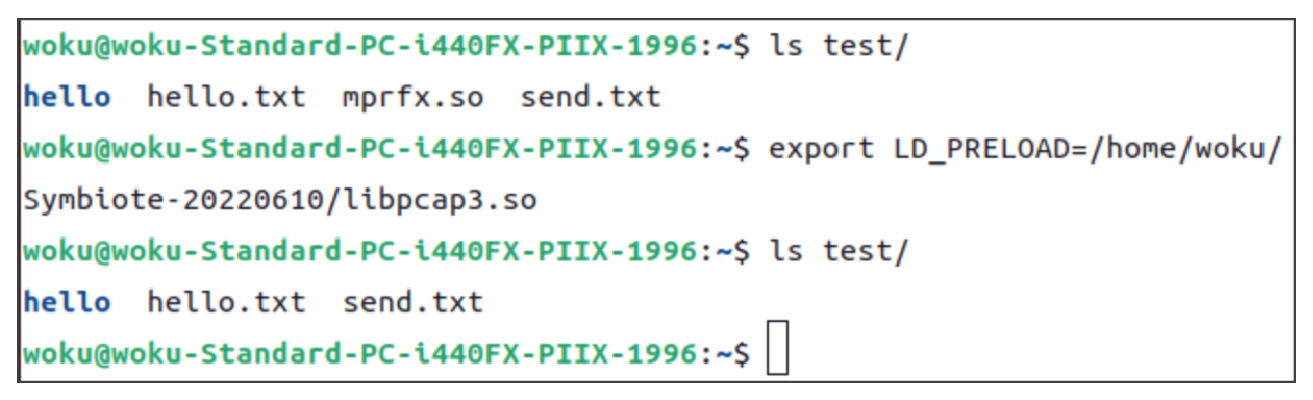
\includegraphics[width=12cm]{fig/ls.eps}
	\caption{ls 実行結果}
	\label{fig:ls}
\end{figure*}

\subsubsection{システムコール}
4.4.1節と同じ条件において,lsコマンドを実行したときのシステムコールをstrace -cで観測する.
readdirは,実行時の条件によって,Symbiteの処理が変化しない.
これを確認するために,Symbioteありの場合について,隠蔽対象のファイル(mprfx.so)がtestディレクトリ内にある場合とない場合の2通りについて収集を行った.
結果を表5にまとめる.Symbiteありの場合は,Symbioteなしの場合に比べて,隠蔽ファイルの有無に関わらずreadlinkシステムコールのみが増えた.
Symbioteありの場合は,処理内容が同じため,システムコールの統計もどちらも全く同じ結果となった.

\subsection{fopen}
\subsubsection{出力結果}
fopenの影響調査のために,fopenを呼び出しファイルの中身を出力する簡単なプログラムfopen.cを作成した.
fopen.cのソースコードを図2に示す.
Symbioteは,fopenで/proc/net/tcpファイルが開かれるとき,置き換え元のfopenを呼び出すことに加えて,tcpの接続状況の隠蔽を行う.
Symbioteの処理が実行される条件を/proc/net/tcpを開くときとして,実験を行う.
fopen.cをgccでコンパイルし,作成したfopen実行ファイルを使用して,それぞれ/proc/net/tcpファイルを出力する.
このとき,どちらの場合もSymbioteによって隠蔽される54778番ポートを使ってローカルホストと接続をしておく.
Symbioteありの実行結果を図3,Symbioteなしの実行結果を図4に示す.
Symbioteなしの場合とありの場合の出力結果を比較すると,Symbioteありのときは1,6,7番目の接続状況が省略されていることがわかる.
これらは全て54778番ポート(16進表記でD5FA番ポート)での接続である.
出力結果としては,割り振られた番号はそのままに,該当するポート番号の情報が出力から省略されることがわかった.\\

\subsubsection{システムコール}
4.5.1節と同じ条件において,fopenを実行したときのシステムコールをstrace -cで観測する.
readdirは,実行時の条件によって,Symbiteの独自の処理が加えられる.
これを確認するために,Symbioteありの場合について,条件を満たす場合(/proc/net/tcpを開く場合)と条件を満たさない場合(/proc/net/udpを開く場合)の2通りについて収集を行った.
結果を表6にまとめる.Symbioteなしの場合とSymbioteあり(条件を満たさない)の場合は,発行されるシステムコールの種類が全く同じ結果となった.
比較して,Symbioteあり(条件を満たす)の場合は,発行されるシステムコールの種類が増加した.
これは,Symbioteの独自の処理が実行されたときに発行されるシステムコールであると考えられる.
この結果から,fopenの実行において,Symbiote感染時にシステムコールの違いを観測できるのは,特定の条件を満たしたときのみであることがわかる.

\begin{figure*}[t]
	\centering
  \includegraphics[width=12cm]{fig/fopen-c.eps}
	\caption{fopen.c}
	\label{fig:fopen.c}
\end{figure*}



\begin{figure*}[t]
	\centering
  \includegraphics[width=12cm]{fig/fopen-0.eps}
	\caption{fopen(Symbioteなし)出力結果}
	\label{fig:fopen0}
\end{figure*}

\begin{figure*}[t]
	\centering
  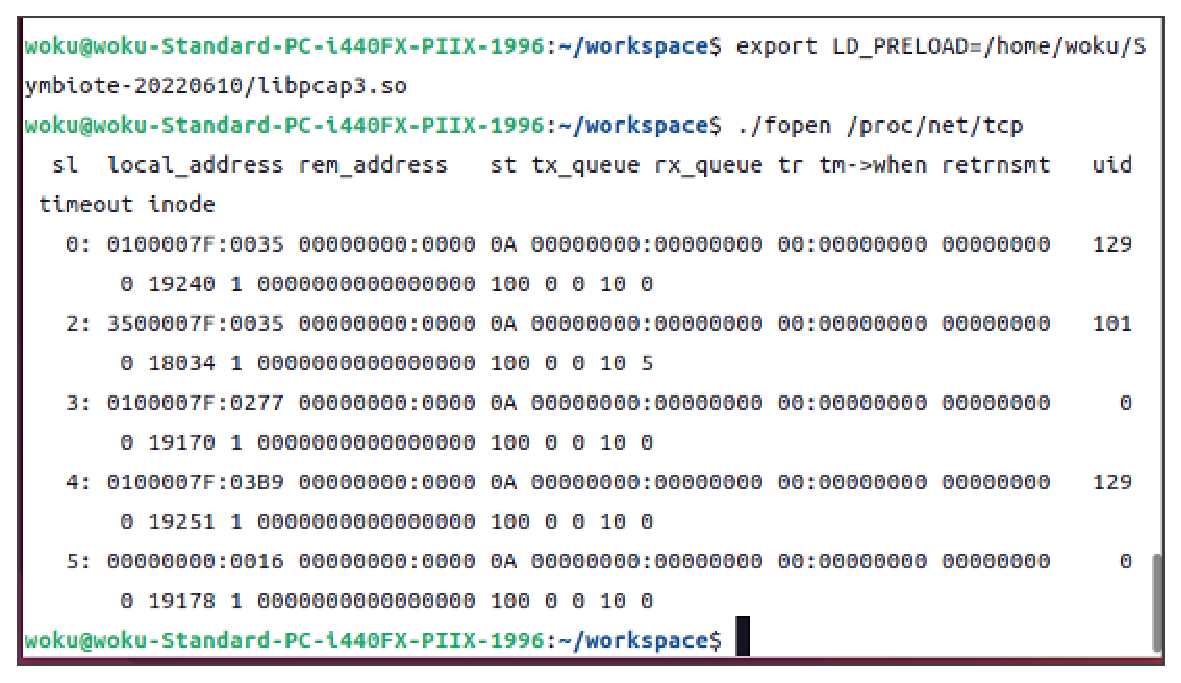
\includegraphics[width=12cm]{fig/fopen-1.eps}
	\caption{fopen(Symbioteあり)出力結果}
	\label{fig:fopen1}
\end{figure*}

\section{おわりに}
共有ライブラリ関数の置き換えを行うLinuxマルウェアであるSymbioteの調査を行なった.
ソースコードの静的解析により,Symbioteのライブラリ関数は,実行されたときの条件によって,処理の内容が変化するものとしないものがあると分かった.
調査を行なった16種類のライブラリ関数において,変化するものが9種類,変化しないものが6種類であった.
また,Symbioteがエクスポートする各ライブラリ関数について,Symbiteなしの場合,Symbiteありで条件を満たす場合,Symbioteありで条件を満たさない場合の3通りのstraceの統計を取得した.
その結果,Symbiote感染時であっても,ライブラリ関数ごとに特定の条件を満たしたときのみ,出力結果やシステムコールに変化が現れる場合があることがわかった.
条件の内容は,攻撃者がリモートログインしているときや,攻撃者と通信を行っているときに,そのことを隠蔽するものが多かった.
よって,それらに関するライブラリ関数の置き換えをシステムコールから確認できるのは,攻撃者による通信やアクセスが行われているときのみであると分かる.

%bibtex
\setlength\baselineskip{12pt}
{\small
	\bibliography{references}
	\bibliographystyle{ipsjunsrt}
}


\end{document}
